\documentclass[12pt, twoside]{article}
\usepackage[letterpaper, margin=1in, headsep=0.2in]{geometry}
\setlength{\headheight}{0.6in}
%\usepackage[english]{babel}
\usepackage[utf8]{inputenc}
\usepackage{microtype}
\usepackage{amsmath}
\usepackage{amssymb}
%\usepackage{amsfonts}
\usepackage{siunitx} %units in math. eg 20\milli\meter
\usepackage{yhmath} % for arcs, overparenth command
\usepackage{tikz} %graphics
\usetikzlibrary{quotes, angles}
\usepackage{graphicx} %consider setting \graphicspath{{images/}}
\usepackage{parskip} %no paragraph indent
\usepackage{enumitem}
\usepackage{multicol}
\usepackage{venndiagram}

\usepackage{fancyhdr}
\pagestyle{fancy}
\fancyhf{}
\renewcommand{\headrulewidth}{0pt} % disable the underline of the header
\raggedbottom
\hfuzz=2mm %suppresses overfull box warnings

\usepackage{hyperref}

\fancyhead[LE]{\thepage}
\fancyhead[RO]{\thepage \\ Name: \hspace{4cm} \,\\}
\fancyhead[LO]{BECA / Dr. Huson / Geometry\\*  Unit 1: Segments, length, and area\\* 22 Sept 2022}

\begin{document}

\subsubsection*{1.9 Homework: Solving for missing parameters} 
\begin{enumerate}
\item The $\triangle DEF$ has an area $A=54$ and base $DE=12$.
  \begin{multicols}{2}
    Find its height, starting with an equation. \\[0.5cm]
    $\displaystyle A = \frac{1}{2} bh = 54$ \vspace{2cm}
      \begin{flushright}
      \begin{tikzpicture}[scale=.635]
        %\draw[help lines] (-1,-1) grid (9,6);
        \draw[thick, ->] (-1.2,0) -- (9.4,0) node [below right]{$x$};
        \draw[thick, ->] (0,-1.2)--(0,6.4) node [left]{$y$};
        \draw[<->, thick] (0.5,1)--(0.5,5);
        \draw[thick] (2,1)--(7,1)--(1,5)--cycle;
        \draw[dashed] (7,1)--(6,5)--(1,5);
        \draw[fill] (2,1) circle [radius=0.05] node[below]{$D$};
        \draw[fill] (7,1) circle [radius=0.05] node[below]{$E$};
        \draw[fill] (1,5) circle [radius=0.05] node[above right]{$F$};
        \node at (4.5,1)[below]{$12$};
        \node at (0.5,3)[right]{$h$};
      \end{tikzpicture}
      \end{flushright}
  \end{multicols}

\item Given circle $O$ with area $A=49 \pi$ square centimeters.
  \begin{multicols}{2}
    Find the radius of circle, $OP$. Start with the formula
    $$A = \pi r^2 = 49 \pi$$ \vspace{2cm}
  \begin{flushright}
    \begin{tikzpicture}[scale=0.8]
      \draw (0,0) circle[radius=3];
      \draw[thick]
      (0:3) node[right]{$P$}--
      (0,0) node[below]{$O$};
      \draw (1.5,0) node[below]{$r=?$};
    \end{tikzpicture}
  \end{flushright}
  \end{multicols}

\item Mark each statement true of false.
\begin{enumerate}[itemsep=0.3cm]
  \item T \quad F \qquad 3.14 is the exact value of $\pi$
  \item T \quad F \qquad $4\pi$ is the area of a circle with radius 2 in terms of $\pi$
  \item T \quad F \qquad $C = 10\pi \approx 31.4$ is an approximation
  \item T \quad F \qquad $3\sqrt{2}$ is an exact value
  \item T \quad F \qquad $0.707$ is an approximation to the \emph{nearest thousandth} for $\displaystyle \frac{1}{\sqrt{2}}$
  \item T \quad F \qquad Rounding 10.498 to the nearest whole number should round up because since 9 is more than 5, first you round to 10.5, then that rounds up to 11.
\end{enumerate}

\newpage
\item One side of the $\triangle ABC$, the base, has a length $AB=8$ centimeters. The triangle's area is 44 square centimeters. Find the height of the triangle, shown as a dashed line in the diagram. \par
\begin{tikzpicture}[scale=1, rotate=-40]
  \draw[thick]
    (2,0)node[below left]{$A$}--
    (8,0)node[below]{$B$}--
    (5,3)node[above]{$C$} --(2,0);
  \draw[dashed] (5,0)--(5,3);
  \draw (5,0)++(0.3,0)--++(0,0.3)--+(-0.3,0);
  \node at (5,1)[right]{$h=?$};
  \node at (5,0)[below left]{$8$};
\end{tikzpicture}

\item Find the area of the shape shown below composed of a rectangle and a semi-circle.
  \begin{flushright}
    \begin{tikzpicture}[scale=.635]
      \draw[help lines] (0,0) grid (10,8);
      \draw[thick, ->] (-1.2,0) -- (10.4,0) node [above right]{$x$};
      \draw[thick, ->] (0,-1.2)--(0,8.4) node [above right]{$y$};
      \foreach \x in {1,...,10}
        \draw[shift={(\x,0)}] (0pt,-3pt)--(0pt,3pt) node[below=5pt]{$\x$};
      \foreach \y in {1,...,8}
        \draw[shift={(0,\y)}] (-3pt,0pt)--(3pt,0pt) node[left=5pt]{$\y$};
      \draw[thick] (1,1)--(6,1)--(6,7)--(1,7)--cycle;
      \draw[thick] (6,1) arc (-90:90:3);
      \draw[fill] (6,4) circle [radius=0.1];
    \end{tikzpicture}
  \end{flushright} \vspace{1cm}

\item The given isosceles $\triangle TUV$ has a base of $TU=50$ meters and a total perimeter of 200 meters. Find $TV$. \par \smallskip
  \begin{tikzpicture}[scale=0.6]
    \draw[thick](0,0)--(4,0)--(2,6)--(0,0);
    \draw[fill] (0,0) circle [radius=0.05] node[below left]{$T$};
    \draw[fill] (4,0) circle [radius=0.05] node[below right]{$U$};
    \draw[fill] (2,6) circle [radius=0.05] node[above left]{$V$};
    \draw[thick] (0.8,3.1)--(1.2,3); %tick mark
    \draw[thick] (2.8,3)--(3.2,3.1); %tick mark
    \node at (2,0) [below]{$50$ m};
    \node at (0.2,3.4){$?$};
    \node at (5,5){$P=200$ m};
  \end{tikzpicture}
  

\end{enumerate}
\end{document}